\section{Representing lexical-semantic resources as Linked Data: \emph{lemon}}

\begin{figure}
 \begin{center}

 	 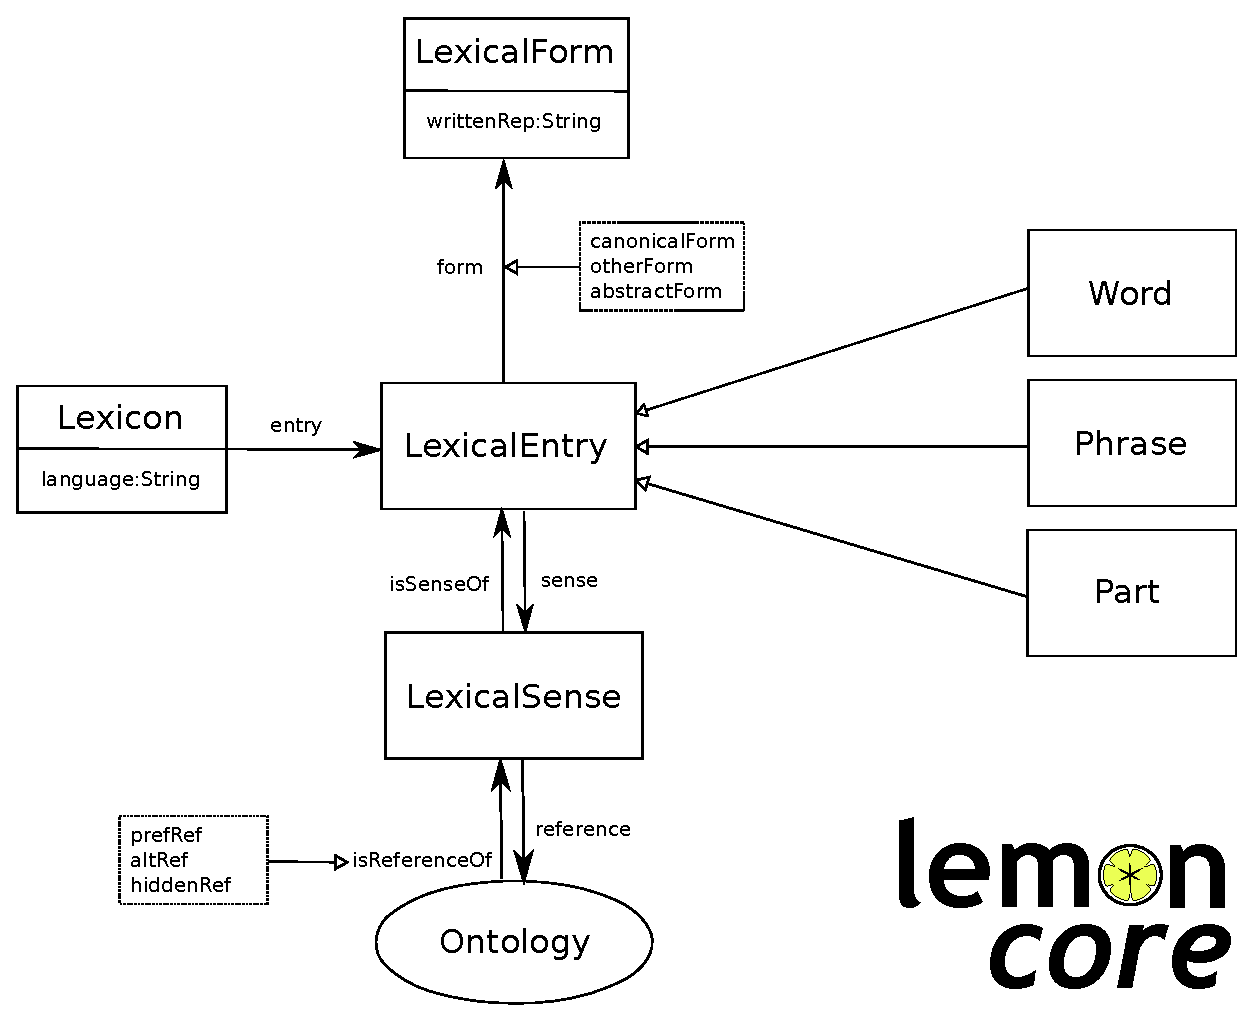
\includegraphics[width=1.0\columnwidth]{images/lemon-core}

 \end{center}
\caption{The core of the \emph{lemon} model\label{lemon-core}}
\end{figure}

\noindent 
There has been significant work towards integrating lexical resources using RDF and
Semantic Web principles~\cite{chiarcos2011towards}, and many resources are already
available as Linked Data. %% CC: less redundant
    % Many lexical resources have already been included in the LLOD cloud, e.g., WordNet, Wikipedia
    % (DBpedia \cite{Bizer_Lehmann_Kobilarov_Auer_Becker_Cyganiak_Hellmann_2009}),
    % and Wiktionary, as well as integrated resources, such as an integrated version of WordNet and Wiktionary\cite{mccrae2012integrating},
    % or of  WordNet and Wikipedia (BabelNet, \cite{navigli2012babelnet}, lexvo?).
    %There has also been some work towards the integration of FrameNet \cite{baker1998berkley} to the Semantic Web \cite{narayanan2003framenet}.
    %All these resources provide a substantial body of lexical knowledge, including semantic relations, multilingual
    %information and encyclopedic knowledge.
Yet, representing lexical resources in RDF does not per se make them semantically
interoperable. Consider, for instance, existing conversions of WordNet and FrameNet \cite{van2006conversion,narayanan2003framenet},
where a simple mapping to RDF is provided, and augmented with OWL semantics so that reasoning could be applied to the structure of the resource.
However, the formats chosen for the RDF versions of WordNet and FrameNet are specific to the underlying data models of WordNet and FrameNet.
    % CC: originally, this sentence mentioned WordNet only, which doesn't make sense as we explicitly announced that we would talk about both WordNet and FrameNet
Although these lexicons are complementary resources~\cite{baker2009wordnet}, % CC: slightly simplified
it is difficult (i) to link them in this form on the Semantic Web, and (ii) to use them as interchangeable modules in NLP applications.

% notably the conversion of WordNet
% \cite{van2006conversion}. They provided a simple mapping from WordNet to RDF, and
% augmented it with OWL semantics so that reasoning could be applied to the structure of the resource.
% Similarly, there has been some work towards mapping
% FrameNet \cite{baker1998berkley} to RDF \cite{narayanan2003framenet}.
% However, the formats chosen for the RDF versions of WordNet and FrameNet are specific to the underlying data models of WordNet
% and FrameNet. Since these lexicons have
% been characterised as complementary resources~\cite{baker2009wordnet}, it is difficult (i) to link the existing versions
% on the Semantic Web, and (ii) to use them as interchangeable modules in NLP applications.

%this resource was specific to the underlying data model of WordNet.
In order to overcome this difficulty, the \emph{lemon} model \cite{mccrae2012interchanging} was proposed
as a common interchange format for lexical resources on the Semantic Web.
\emph{lemon} has its historical roots in LMF and thus allows 
    %% CC: "having roots in" is not causal, merely circumstantial, hence, not "to allow"
easy conversion from LMF-like, non-linked data resources. 
    %% CC: From a SW perspective, one could simply call these "legacy resources", but I guess Judith wouldn't like that too much ;)
It links to data categories in
  annotation terminology repositories, and most of all,
  it realises a separation of lexicon and ontology layers, so that \emph{lemon} lexica can be linked to existing ontologies
in the linked data cloud.


% that supports publishing
% lexical-semantic resources as linked data on the basis of the following principles:
%
% \begin{description}
% \item[LMF-based]: To allow easy conversion from non-linked data resources.
% \item[RDF-native]: Publishing as linked data, with RDFS and OWL used to describe
%   the semantics of the model.
% \item[Modular]: Separation of lexicon and ontology layers, so that \emph{lemon} lexica can be linked to existing ontologies
% in the linked data cloud.
% \item[Externally defined data categories]: Linking to data categories in
%   annotation terminology repositories, rather than being limited to a specific part-of-speech tag set.
% \item[Principle of least power]: The smaller the model and the less expressive the language,
% 	the wider its adoption and the higher the reusability of the
% 	data\cite{shadbolt2006semantic}.
% \end{description}

This core model is illustrated in Fig.\ \ref{lemon-core}, which defines the
basic elements used by all lexica published as linked data. In addition to this there
are a number of modules used to model linguistic description, syntax, morphology
and relationships between lexica.\footnote{More detail of the model and descriptions of
the modules can be found at \url{http://lemon-model.net}}

\emph{lemon} has been used as a basis for integrating the data of the
English Wiktionary
    % \footnote{A (human-readable) dictionary created along wiki principles, see \url{http://www.wiktionary.org}} 
    %% CC: has been introduced in Sect. 1 already
with
the RDF version of WordNet \cite{mccrae2012integrating}.
\emph{lemon}'s similarity
to the WordNet model made this conversion straight-forward, with only the need for
a slight change in modelling to accommodate inflectional variants of lexical
entries.

